\chapter{Strumenti utilizzati}

	\section{Maven}
		Maven è stato utilizzato per gestire le varie dipendenze del progetto e la build automatica.
		Le dipendenze necessarie al programma e quindi inserite nel fatJar sono: 
		\begin{itemize}
			\item \emph{Guava}: libreria di GOOGLE che fornisce un hashmap bidirezionale
			\item \emph{Log4J}: framework per il logging (non realmente necessario ma utilizzato dal Main per stampare messaggi a schermo)
		\end{itemize}
		
	\section{GitHub}
		Il progetto è raggiungibile a questo link https://github.com/ma-buracchi/TAPciphers. 
		
		Inizialmente, per prendere dimestichezza con il processo di branching e di pull request, le classi Shift, Substitution e InputManager sono state create appunto su tre branch diversi e riportate sul ramo master tramite una merge di tre pull request. Essendo comunque un progetto svolto da una singola persona, le rimanenti classi sono state sviluppate direttamente sul ramo master. Un'eccezione è stata fatta per questa relazione, sviluppata su un altro ramo e successivamente mergiata sul ramo master sempre tramite pull request.	
		
	\section{Travis}
		Travis viene utilizzato per la continuous integration. Il relativo file di configurazione è stato settato per utilizzare la jdk8 necessaria alla compilazione del progetto e per fornire il risultato della code coverage a coveralls.
		
		Una build automatica viene lanciata ad ogni push effettuata sul repository GitHub contenente il progetto.
		
		Il progetto è raggiungibile al seguente link: https://travis-ci.org/ma-buracchi/TAPciphers
		
	\section{Coveralls}
		Coveralls riceve i dati della coverage direttamente da Travis.
		
		\begin{figure}[h]
			\centering
			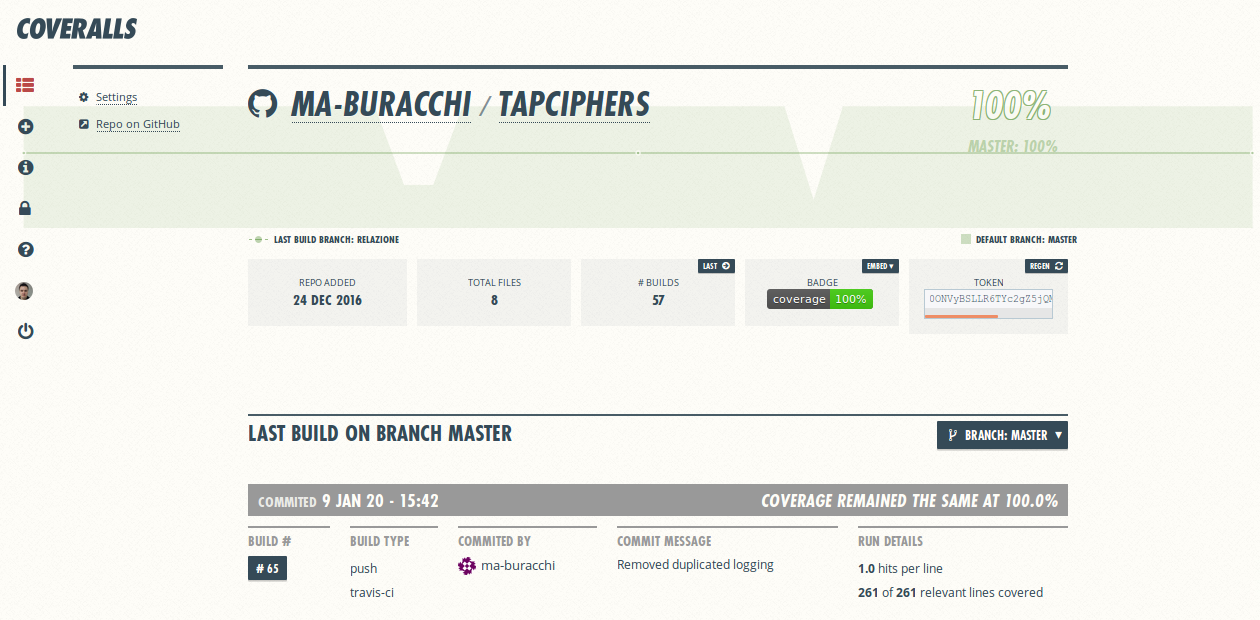
\includegraphics[scale=0.2]{img/coverall}
			\caption{Risultati di Coveralls}
			\label{fig:coveralls}
		\end{figure}
				
		I risultati della code coverage sono visibili al link https://coveralls.io/github/ma-buracchi/TAPciphers.
		
	\section{Docker}
		L'utilizzo di Docker è quello di usare docker-compose per gestire il server di SonarQube senza doverlo effettivamente scaricare. 
		
	\section{Sonarqube}
		Sonarqube viene utilizzato tramite docker compose. E' stata scaricata l'ultima versione, attivando tutte le 395 regole disponibili per Java ad esclusione di quelle presenti in figura \ref{fig:sonarules}
		
		\begin{figure}[h]
			\centering
			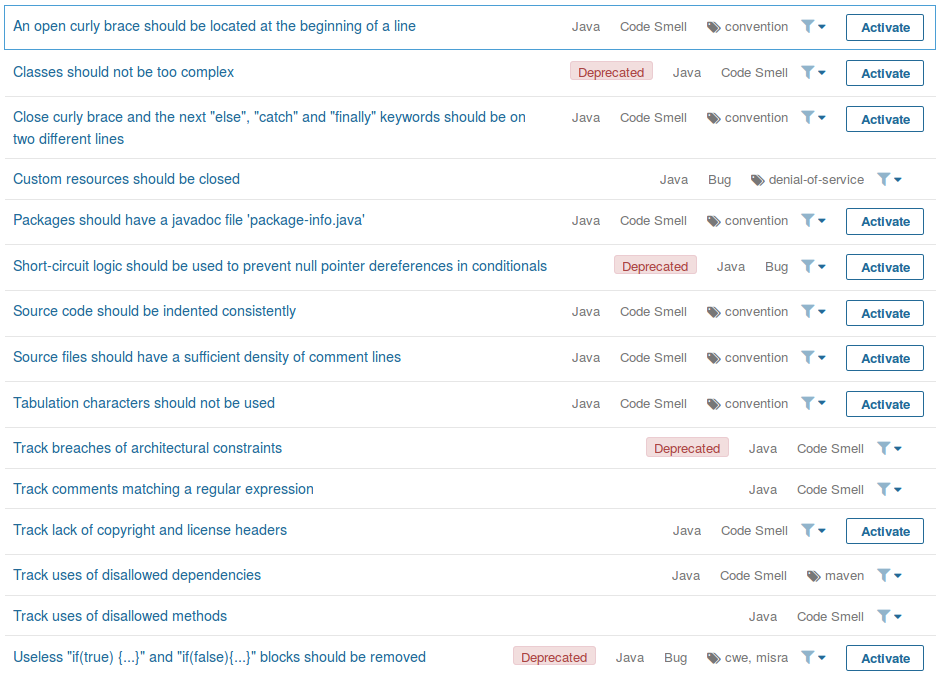
\includegraphics[scale=0.4]{img/sonarqube_rules}
			\caption{Regole disattivate}
			\label{fig:sonarules}
		\end{figure}
		
		Sono state escluse 
		\begin{itemize}
			\item le regole deprecate
			\item le regole riguardanti JavaDoc che non viene utilizzato in quanto questo progetto è pensato per un utilizzo personale e non per essere divulgato
			\item le regole che contestano l'assenza delle informazioni di copyright e di licenza (come sopra)
			\item alcune regole ambigue di formattazione come ad esempio quella che impone di mettere la parentesi graffa aperta di inizio blocco in una nuova linea che contrasta con quella che suggerisce di metterla sulla stessa riga (e con la formattazione di \emph{Eclipse})
		\end{itemize}
		
		Il risultato della scansione utilizzando questi parametri è illustrato in figura \ref{fig:sonaresult}
		
		\begin{figure}[h]
			\centering
			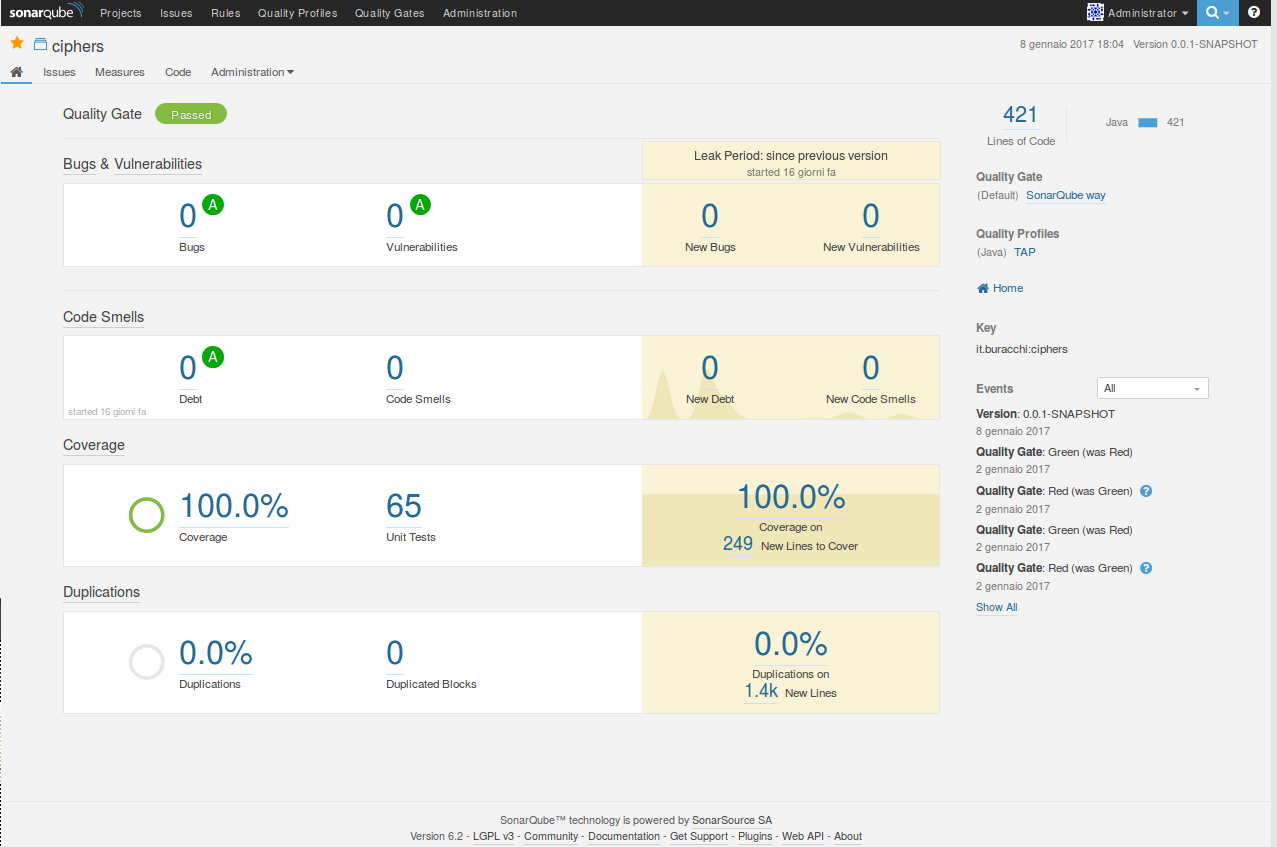
\includegraphics[scale=0.3]{img/sonaresult}
			\caption{Risultato della scansione}
			\label{fig:sonaresult}
		\end{figure}
		